%%%%%%%%%%%%%%%%%%%
% CLAUSE SPLITTING
%%%%%%%%%%%%%%%%%%%

\def\title{Atomic Clauses from Sentences}
\begin{frame}[t]{\title}
\begin{tabular}{ll}
\hh{Input:}  & Long sentence. \\
             & \w{Born in a small town, she took the midnight} \\
             & \w{train going anywhere.} \\
\hh{Output:} & Short clauses. \\
             & \w{she was born in a small town.}
\end{tabular}

\begin{center}
  \only<1>{\treeBlank}
  \only<2>{\hspace{-1ex}\treeEdge}
  \only<3>{\hspace{-1.5ex}\treeSubj}
\end{center}
\end{frame}

%%%%%%%%%%%%%%%%%%%
% CLAUSE SEARCH
%%%%%%%%%%%%%%%%%%%
\def\title{Clause Classifier}
\begin{frame}{\title}
\begin{center}
  \only<1>{\begin{minipage}[t][3.5cm]{\textwidth}               \begin{center}\treeSubj     \end{center}\end{minipage}}
  \only<2>{\hspace{-1.0ex}\begin{minipage}[t][3.5cm]{\textwidth}\begin{center}\treeYield    \end{center}\end{minipage}}
  \only<3>{\hspace{-1.5ex}\begin{minipage}[t][3.5cm]{\textwidth}\begin{center}\treeYieldSubj\end{center}\end{minipage}}
  \only<4>{\hspace{-2.0ex}\begin{minipage}[t][3.5cm]{\textwidth}\begin{center}\treeYieldObj \end{center}\end{minipage}}
  \only<5>{\hspace{-2.5ex}\begin{minipage}[t][3.5cm]{\textwidth}\begin{center}\treeYieldRoot\end{center}\end{minipage}}
\end{center}

\vspace{-.5cm}
\begin{tabular}{ll}
\hh{Input:}  & Dependency arc. \\
\hh{Output:} & \textit{Action} to take.  \\
\end{tabular}
\pause

\begin{itemize}
  \item \textbf{Yield} (\w{you should brush your teeth}) \pause
  \item \textbf{Yield (Subject Controller)} (\w{Obama Born in Hawaii}) \pause
  \item \textbf{Yield (Object Controller)} (\w{Fred leave the room}) \pause
  \item \textbf{Yield (Parent Subject)} (\w{Obama is our 44th president})
\end{itemize}
\end{frame}

%%%%%%%%%%%%%%%%%%%
% TRAINING DATA
%%%%%%%%%%%%%%%%%%%
\def\title{Classifier Training}
\begin{frame}{\title}
\hh{Training Data Generation}
\begin{enumerate}
  \item Label the Penn Treebank with Open IE triples using traces.
  \item Run exhaustive search over possible clause splits.
  \pause
  \item \darkgreen{Positive Labels}: A sequence of actions which yields a relation
                                     (33.5k examples). \\
        \darkred{Negative Labels}: All other sequences of actions (1.1M examples).
\end{enumerate}
\hspace{0.5em}
\pause

\hh{Features:}
\begin{itemize}
  \item Edge label; incoming edge label.
  \item Neighbors of governor + dependent; number of neighbors.
  \item Existence of subject/object edges at governor; dependent.
  \item POS tag of governor; dependent.
\end{itemize}
\end{frame}



%%%%%%%%%%%%%%%%%%%
% MAXIMALLY SHORTEN CLAUSES
%%%%%%%%%%%%%%%%%%%
\def\title{Maximally Shorten Clauses}
\begin{frame}{\title}
\only<1>{\hh{\strut Some strange, nuanced function:}}
\only<2>{\hh{\strut An entailment function:}}
\only<3>{\hh{\strut A \darkblue{natural logic} entailment function:}} \\
\vspace{1em}

\begin{tabular}{lcl}
  \w{Heinz Fischer \textbf{of Austria}}      & $\implies$ & \true{Heinz Fischer} \\
  \w{\textbf{United States president} Obama} & $\implies$ & \true{Obama} \\
  \w{All \textbf{young} rabbits drink milk}  & \darkred{$\centernot \implies$} & \false{All rabbits drink milk} \\
  \w{Some \textbf{young} rabbits drink milk} & $\implies$ & \true{Some rabbits drink milk} \\
  \w{Enemies give \textbf{fake} praise}      & \darkred{$\centernot \implies$} & \false{Enemies give praise} \\
  \w{Friends give \textbf{true} praise}      & $\implies$ & \true{Friends give praise} \\
\end{tabular}
\end{frame}


%%%%%%%%%%%%%%%%%%%
% NATURAL LOGIC FOR DELETIONS
%%%%%%%%%%%%%%%%%%%
\def\title{Natural Logic For Clause Shortening}
\def\some{\monoUp{}{\textbf{Some$_{\uparrow \uparrow}$}}{}{}}
\def\rabbits{\monoUp{baby rabbits}{\footnotesize{young rabbits}}{rabbits}{mammals}}
\def\drink{\monoUp{slurp}{drink}{consume}{}}
\def\milk{\monoUp{Lucerne}{milk}{liquid}{something}}
\def\all{\monoUp{}{\textbf{All$_{\downarrow \uparrow}$}}{}{}}
\def\cats{\monoDown{house cats}{cats}{felines}{carnivores}}
\def\eat{\monoUp{slurp}{eat}{consume}{}}
\def\mice{\monoUp{fieldmice}{mice}{rodents}{placentals}}

\begin{frame}[noframenumbering]{\title}
\hh{Quantifiers determines the \textit{polarity} ($\uparrow$ or $\downarrow$) of words.} \\
\vspace{0.25cm}
\hh{Mutations must respect \textit{polarity}.} \\
\vspace{0.25cm}
\hh{Polarity determines valid deletions.}
\vspace{0.5cm}
\begin{center}
  \some \hspace{0.25cm} \rabbits \hspace{0.25cm} \drink \milk
\end{center}
\end{frame}

\def\rabbits{\monoUp{\footnotesize{young rabbits}}{\darkgreen{rabbits}}{mammals}{animals}}
\begin{frame}[noframenumbering]{\title}
\hh{Quantifiers determines the \textit{polarity} ($\uparrow$ or $\downarrow$) of words.} \\
\vspace{0.25cm}
\hh{Mutations must respect \textit{polarity}.} \\
\vspace{0.25cm}
\hh{Polarity determines valid deletions.}
\vspace{0.5cm}
\begin{center}
  \some \hspace{0.25cm} \rabbits \hspace{0.25cm} \drink \milk
\end{center}
\end{frame}

\def\rabbits{\monoDown{baby rabbits}{\footnotesize{young rabbits}}{rabbits}{mammals}}
\begin{frame}[noframenumbering]{\title}
\hh{Quantifiers determines the \textit{polarity} ($\uparrow$ or $\downarrow$) of words.} \\
\vspace{0.25cm}
\hh{Mutations must respect \textit{polarity}.} \\
\vspace{0.25cm}
\hh{Polarity determines valid deletions.}
\vspace{0.5cm}
\begin{center}
  \all \hspace{0.25cm} \rabbits \hspace{0.25cm} \drink \milk
\end{center}
\end{frame}

\def\rabbits{\monoDown{\footnotesize{young rabbits}}{\darkred{rabbits}}{mammals}{animals}}
\begin{frame}[noframenumbering]{\title}
\hh{Quantifiers determines the \textit{polarity} ($\uparrow$ or $\downarrow$) of words.} \\
\vspace{0.25cm}
\hh{Mutations must respect \textit{polarity}.} \\
\vspace{0.25cm}
\hh{Polarity determines valid deletions.}
\vspace{0.5cm}
\begin{center}
  \all \hspace{0.25cm} \rabbits \hspace{0.25cm} \drink \milk
\end{center}
\end{frame}


%%%%%%%%%%%%%%%%%%%
% TRIPLES
%%%%%%%%%%%%%%%%%%%
\def\title{Bonus: Knowledge Base Triples}
\begin{frame}{\title}
\begin{center}
\begin{tabular}{lcl}
  \w{Heinz Fischer visited US} & $\implies$ & 
    \triple{Heinz Fischer}{visited}{US} \\\pause
  \w{Obama born in Hawaii} & $\implies$ & 
    \triple{Obama}{born in}{Hawaii} \\\pause
  \w{Cats are cute} & $\implies$ & 
    \triple{Cats}{are}{cute} \\\pause
  \w{Cats are sitting next to dogs} & $\implies$ & 
    \triple{Cats}{are sitting next to}{dogs} \\\pause
    & $\dots$ & 
\end{tabular}
\vspace{2em}

\hh{5 dependency tree patterns (+ 8 nominal patterns)}
\end{center}
\end{frame}

%%%%%%%%%%%%%%%%%%%
% EVALUATION
%%%%%%%%%%%%%%%%%%%
\def\title{Extrinsic Evaluation: Knowledge Base Population}
\begin{frame}[noframenumbering]{\title}
\begin{center}
\begin{tabular}{cccc}
  \begin{tabular}{c}
    \h{Unstructured Text} \\
    \\
    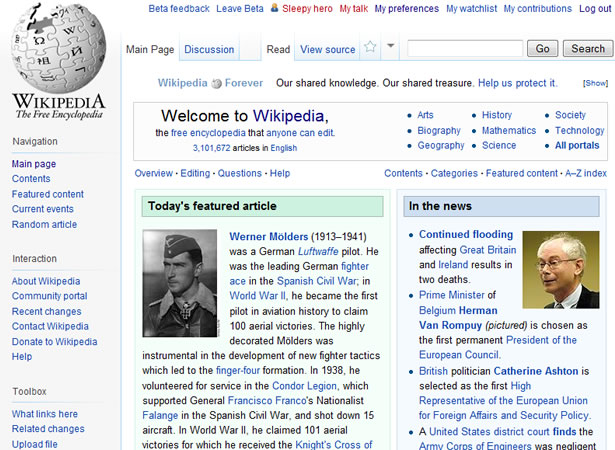
\includegraphics[width=2cm]{../img/wiki.jpg} \\
    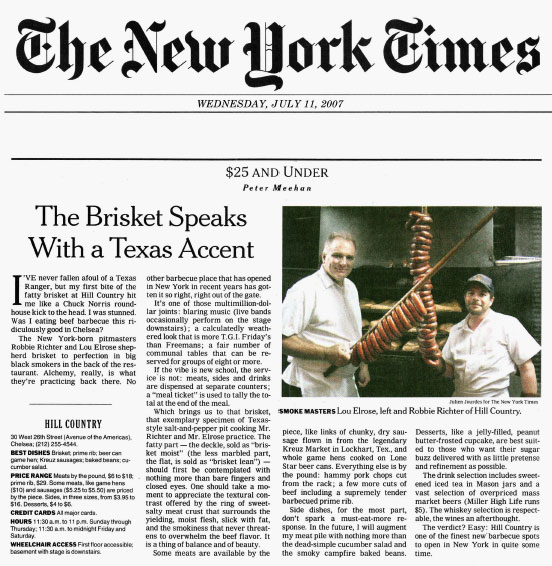
\includegraphics[width=2cm]{../img/nyt.jpg} \\
    
\includegraphics[width=2cm]{../img/blog.jpg}
  \end{tabular} &

  \Huge{$\Rightarrow$} &
  
  \begin{tabular}{c}
  \h{Structured Knowledge Base} \\
  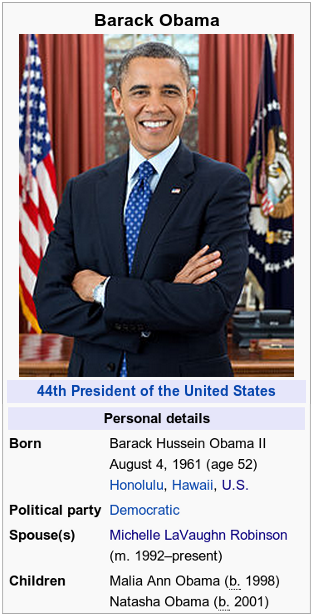
\includegraphics[width=2.75cm]{../img/obama-infobox.png}
  \end{tabular}
\end{tabular}
\end{center}
\end{frame}

\begin{frame}[noframenumbering]{\title}
\hh{Relation Extraction Task:}
\begin{itemize}
  \item Fixed schema of 41 relations.
  \item Precision: answers marked correct by humans.
  \item Recall: answers returned by any team (including LDC annotators).
\end{itemize}
\pause
\vspace{1em}

\hh{Comparison:} \textit{Open Information Extraction to KBP Relations in 3 Hours}.
  \cite{key:2013soderland-kbp}

\begin{center}
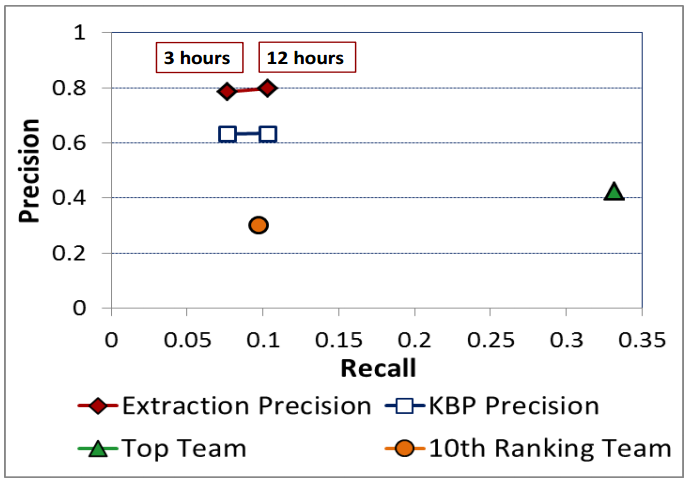
\includegraphics[scale=0.20]{../img/uw-openie.png} \\
\end{center}
\end{frame}

%%%%%%%%%%%%%%%%%%%
% RELATION MAPPING
%%%%%%%%%%%%%%%%%%%
\def\title{Prerequisite Task: Text $\rightarrow$ KBP Relations}
\begin{frame}{\title}
\begin{enumerate}
  \item Hand-coded mapping. \\
        (Same as UW; both over 1-2 weeks)
        \pause
        \vspace{1em}

  \item Learned relation mapping.
  \begin{itemize}
    \item For each type signature $t_1, t_2$;
    \item For an text relation $r_o$ and KBP relation $r_k$;
    \pause
    \item Compute:
      \begin{center}
        $
        p(r_k, r_o \mid t_1, t_2) = \frac{
          \textrm{count}(r_k, r_o,  t_1, t_2)
        }{
          \sum_{r_k', r_o'}\textrm{count}(r_k', r_o', t_1, t_2)
        }
        $.
      \end{center}
    \pause
    \item Rank by PMI$^2(r_o, r_k \mid t_1, t_2)$:
      \begin{center}
        $
        \textrm{PMI}^2(r_k, r_o \mid t_1, t_2) = \log \left( \frac{p(r_k, r_o \mid t_1, t_2)^2}{p(r_k \mid t_1, t_2) \cdot p(r_o \mid t_1, t_2)} \right)
        $.
      \end{center}
  \end{itemize}
\end{enumerate}
\end{frame}


%%%%%%%%%%%%%%%%%%%
% Map to KB
%%%%%%%%%%%%%%%%%%%
\def\title{Map Triples to Structured Knowledge Base}
\begin{frame}{\title}
\begin{center}
\begin{tabular}{l:lc}
  \textbf{KBP Relation} & \textbf{Text} & \textbf{PMI$^2$}\\
  \hline
  \small{\rel{Per:Date\_Of\_Birth}}    & \ww{be bear on} & 1.83       \\
                                       & \ww{bear on} & 1.28          \\
  \small{\rel{Per:Date\_Of\_Death}}   & \ww{die on} & 0.70  \\
                                      & \ww{be assassinate on} & 0.65  \\
  \small{\rel{Per:LOC\_Of\_Birth}}     & \ww{be bear in} & 1.21        \\
  \small{\rel{Per:LOC\_Of\_Death}}     & \ww{\darkred{*elect president of}} & 2.89                \\
  \small{\rel{Per:Religion}}          & \ww{speak about} & 0.67   \\
                                      & \ww{popular for} & 0.60   \\
  \small{\rel{Per:Parents}}            & \ww{daughter of}     & 0.54          \\
                                      & \ww{son of} & 1.52          \\
  \small{\rel{Per:LOC\_Residence}}     & \ww{of} & 1.48       \\
                                       & \ww{\darkred{*independent from}} & 1.18    \\
\end{tabular}
\end{center}
\end{frame}


%%%%%%%%%%%%%%%%%%%
% RESULTS
%%%%%%%%%%%%%%%%%%%
\def\title{Results}
\begin{frame}{\title}
\hh{TAC-KBP 2013 Slot Filling Challenge:}
\begin{itemize}
  \item End-to-end task: includes IR + consistency.
\item \textbf{Precision:} facts LDC evaluators judged as correct. \\
      \textbf{Recall:} facts other teams (including LDC annotators) also found.
\end{itemize}
\vspace{0.25cm}

\def\bell{\raisebox{-2.5mm}{
\includegraphics[height=5mm]{../img/bell.png}}}
\def\whistle{\raisebox{-2.5mm}{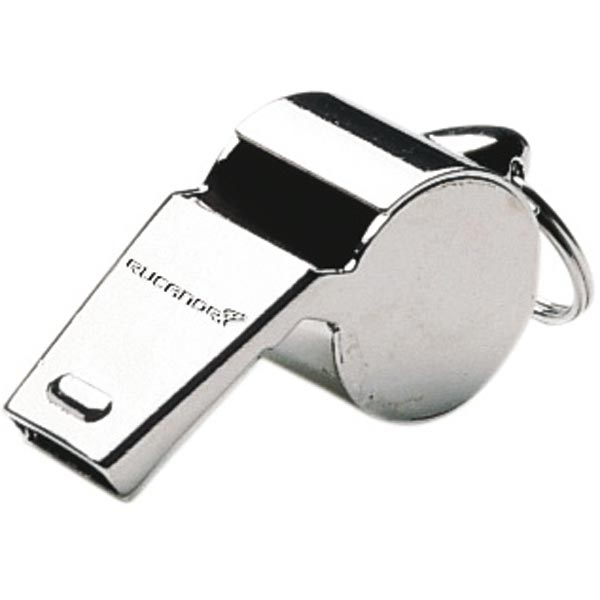
\includegraphics[height=5mm]{../img/whistle.jpg}}}
\begin{center}
\begin{tabular}{lrrr}
\hline
\textbf{System}                & \multicolumn{1}{c}{\textbf{P}}    
                               & \multicolumn{1}{c}{\textbf{R}}    
                               & \multicolumn{1}{c}{\textbf{F$_1$}} \\
\hline
UW Submission                   & 69.8          & 11.4          & 19.6 \\
Ollie                           & 57.7          & 11.8          & 19.6 \\
\pause
\darkblue{Our System}           & \darkblue{61.9} & \darkblue{13.9} & \darkblue{22.7} \\
\hline
\pause
Median Team                     &               &               & 18.6 \\
\darkblue{Our System} + \bell\ + \whistle  & \darkblue{58.6} & \darkblue{18.6} & \darkblue{28.3} \\
Top Team                        & 45.7          & 35.8          & 40.2 \\
\hline
\end{tabular}
\end{center}
\end{frame}
